% Name: Timing diagram
% Description: A clock, a data input, and a flip-flop output that changes only on rising clock edges.
% Tags: timing diagram, flip-flop, clock, waveform

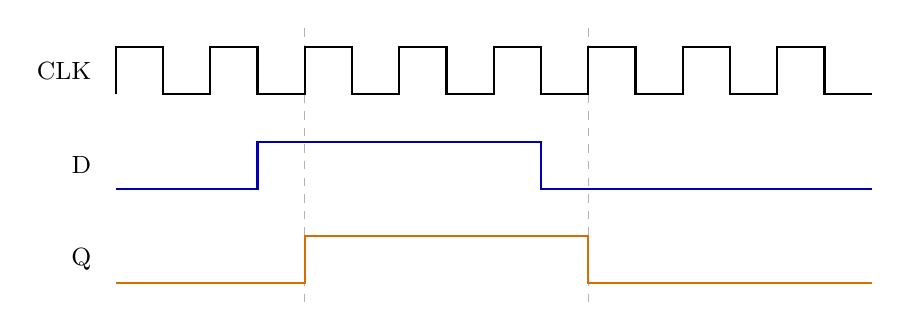
\begin{tikzpicture}[x=6mm, y=6mm, thick, every node/.style={font=\small}]
  \foreach \x in {4, 10}
    \draw[gray!60, dashed, thin] (\x,1.4) -- (\x,-4.4);
  \node[left] at (-0.3,0.5) {CLK};
  \draw (0,0) \foreach \i in {0,...,7} { -- ++(0,1) -- ++(1,0) -- ++(0,-1) -- ++(1,0) };
  \node[left] at (-0.3,-1.5) {D};
  \draw[blue!70!black] (0,-2) -- (3,-2) -- (3,-1) -- (9,-1) -- (9,-2) -- (16,-2);
  \node[left] at (-0.3,-3.5) {Q};
  \draw[orange!85!black] (0,-4) -- (4,-4) -- (4,-3) -- (10,-3) -- (10,-4) -- (16,-4);
\end{tikzpicture}
